%# -*- coding: utf-8-unix -*-
%%==================================================
\chapter{量子力学基础}

\section{微观粒子的运动特征}
经典物理学的三大支柱
\begin{itemize}
\item Newton 经典力学
\item Maxwell 电磁理论
\item Boltzman和Gibbs 统计力学
\end{itemize}

经典物理学的困难
\begin{itemize}
\item \qd{黑体辐射}(经典物理的天空的两朵乌云之一)
\item \qd{光电效应}
\item 原子的稳定性和原子的光谱线
\item 低温下,固体的比热问题
\item $\cdots \cdots$
\end{itemize}


\subsection{黑体辐射和能量量子化}

\begin{defT}[黑体]
黑体是一种能全部吸收照射到它上面的各种波长辐射的物体。
\end{defT}
黑体是理想的吸收体,也是理想的发射体。

\begin{exT}
带有一微孔的空心金属球,从小孔进入金属球内部的辐射,经过多次吸收、反射、使射入的辐射实际上全部被吸收。当空腔受热时,空腔壁会发出辐射,极小部分通过小孔逸出。这样的空心金属球非常接近于黑体。
\end{exT}

初步尝试:
\begin{itemize}
\item Wien:热力学 $\rightarrow$ Wien公式 $\rightarrow$ 长波区不符,失败!
\item Rayleigh:电动力学 $\rightarrow$ Rayleigh-Jeans公式 $\rightarrow$ 短波区不符,导致所谓“紫外灾变”,失败!
\end{itemize}

为了解决黑体辐射的问题,\planck 被迫假设黑体吸收或发射辐射的\qd{能量必须是不连续的,即量子化的}。辐射能量的最小单元为$h\nu$,$\nu$是振子的频率,$h$ 就是著名的Planck常数:$ 6.626 \times 10^{-34} J \cdot s$。
\qd{$$ \rho = \frac{8\pi h c}{\lambda ^ 5} \left( \frac{1}{exp(hc/\lambda k T) - 1} \right) $$}

\begin{figure}[!ht]
\centering
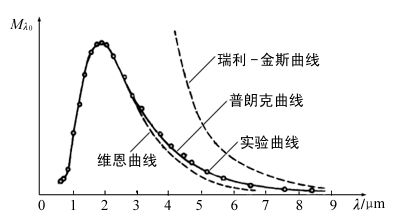
\includegraphics[height=5cm]{pic/black_body_radiation_lambda.jpg}
\caption{Wien公式、Rayleigh-Jeans公式、\planck 公式、及黑体辐射的实验曲线}
\end{figure}

\begin{figure}[!ht]
\centering
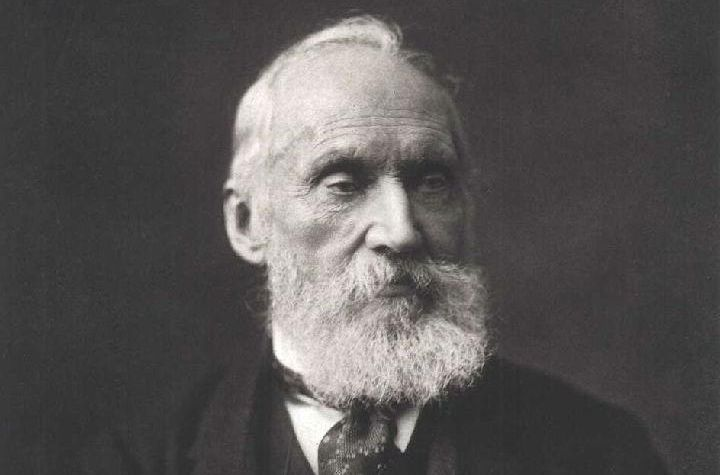
\includegraphics[height=5cm]{pic/Kelvine.jpg}
\caption{\kelv 爵士,原名William Thomson}
\end{figure}

\begin{figure}[!ht]
\centering
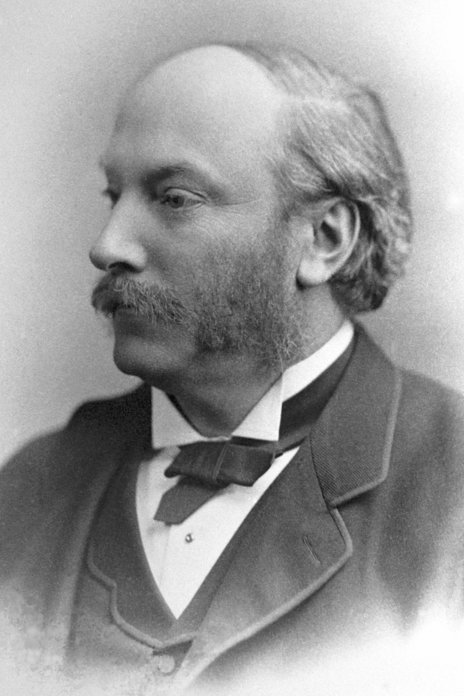
\includegraphics[height=7cm]{pic/Rayleigh.jpg}
\caption{\rayleigh 爵士,原名John William Strutt,1904年诺贝尔物理奖}
\end{figure}

\begin{figure}[!ht]
\centering
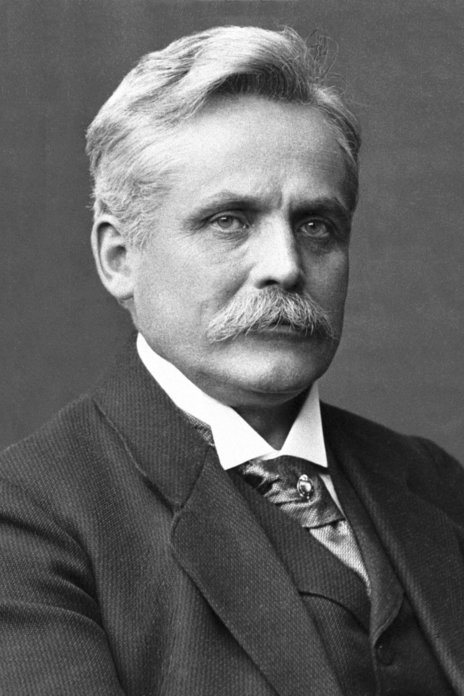
\includegraphics[height=7cm]{pic/Wien.jpg}
\caption{\wein,1911年诺贝尔物理奖}
\end{figure}

\begin{figure}[!ht]
\centering
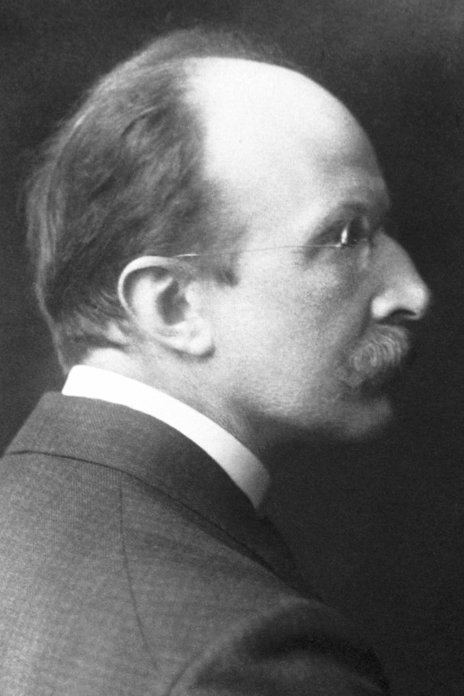
\includegraphics[height=7cm]{pic/Planck.jpg}
\caption{\planck,1918年诺贝尔物理奖}
\end{figure}



\subsection{光电效应和光子学说}
大家在中学物理课程中都接触过光电效应,这里回顾光电效应的一些重要事实:
\begin{itemize}
\item 只有当照射光的频率超过某个最小频率(即临阈频率)时,金属才能发射光电子,不同金属的临阈频率不同。
\item 随着光强的增加,发射的电子数也增加,但不影响光电子的动能。
\item 增加光的频率,光电子的动能也随之增加。
\end{itemize}

\begin{figure}[!ht]
\centering
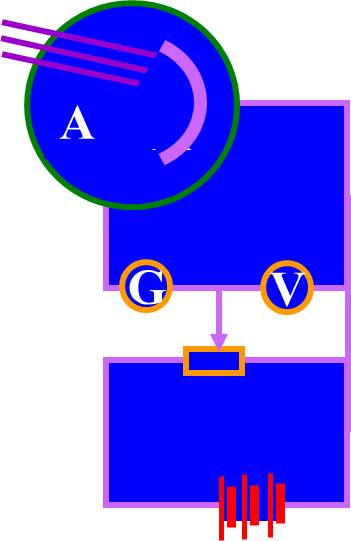
\includegraphics[height=10cm]{pic/photon_electron.jpg}
\caption{光电效应示意图}
\end{figure}

\qd{经典物理的困难}:光电子的动能显然来自光能。按照经典波动理论,光能取决于光强度即振幅平方而与频率无关。显然, 经典波动理论完全不能解释光电效应的实验事实!

1905年, \einstein 提出光量子(光子)概念,将光解释为光子的集合,成功地解释了光电效应。给出了光电效应方程$$\frac{1}{2}mv^2=h\nu - \phi,$$ 其中$\nu$为光子的频率,$\phi$为金属的功函数(脱出功)。 
显然,将动能$\frac{1}{2}mv^2$对$\nu$作图将得到一条截距为$-\phi$的直线。当光的频率小于阈值$\nu_0 = \phi / h$时,动能为负,此时无光电子产生。

\einstein 光子学说要点:
\begin{itemize}
\item 光是一束光子流,每一种频率的光的能量都有一个最小单位,称为光的量子或光子。光子的能量与光子的频率成正比,即$\epsilon = h\nu$。
\item 光子不但有能量($\epsilon$),还有质量(m),但光子的静止质量为零。按相对论的质能方程$ \epsilon = mc^2$,光子的质量$ m = \epsilon/c^2 = h\nu/c^2 $,所以不同频率的光子有不同的质量。
\item 光子具有一定的动量,$ p = mc = h\nu/c = h / \lambda $。
\item 光子的强度取决于单位体积内光子的数目,即光子的密度。		
\end{itemize}
光子学说表明了光不仅有波动性,且有微粒性,这就是光的\qd{波粒二象性}思想。


\subsection{$^\star$氢原子光谱和Bohr理论}
\bohr 之前人们对氢原子光谱的认识:
\begin{itemize}
\item 1885年Balmer线系:$\nu_n=R(\frac{1}{2^2}-\frac{1}{n^2})$,R为Rydberg常数
\item 1889年Rydberg方程:$\nu_{n1,n2}=R(\frac{1}{n_1^2}-\frac{1}{n_2^2})$
\item 1908年在近红外区发现了Paschen线系($n_1=3$)
\item 1914年在紫外区发现了Lyman线系($n_1=1$)
\item 1922年在红外区发现Brackett线系($n_1=4$)
\item 1924年在远红外区发现Pfund线系($n_1=5$)
\end{itemize}

\begin{figure}[!ht]
\centering
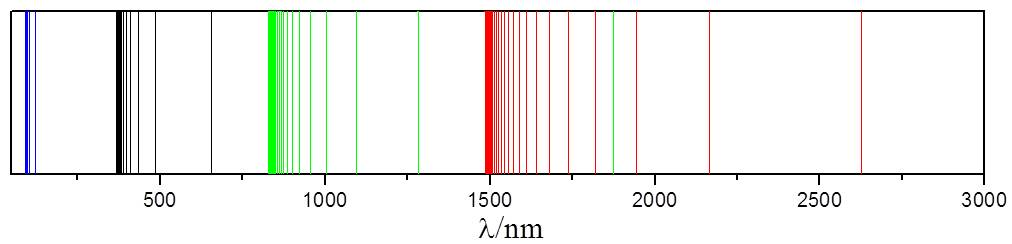
\includegraphics[width=\textwidth]{pic/H_spectroscopy.jpg}
\caption{氢光谱示意图}
\end{figure}

\begin{statT}[Bohr理论要点]
\bohr 于1913年基于Rutherford提出的原子模型,综合\planck 和\einstein 的量子论,提出了关于原子结构的模型。其要点如下:
\begin{itemize}
\item 经典轨道加定态条件
\small{氢原子中的电子绕原子核作圆周轨道运动,在一定轨道运动的电子具有一定的能量,电子若不发生跃迁,总是处于定态,处于定态时的原子不产生辐射,根据核对电子的静电引力与电子在轨道上运动的离心效应的平衡,可以求出允许的定态。}

\item 频率条件
\small{原子从一个定态跃迁到另一个定态要吸收或发射频率为$\nu$的辐射,其频率条件由$ h\nu = E_2 - E_1 $决定。}

\item 角动量量子化
\small{对于原子各种可能存在的定态有一个限制,即电子轨道运动的角动量必须等于$\hbar(=h/2\pi)$的整数倍。}
\end{itemize}
\end{statT}

根据以上假定,计算氢原子电子绕核运动的半径$ a_0 = 52.92 pm$ (\bohr 半径),所计算出Rydberg常数与实验完全吻合。
\bohr 于1922年获得Nobel物理奖。

\subsection{实物粒子的波粒二象性}
实物微粒的波粒二象性:
1924年,\deB 认为辐射的波粒二象性同样适用于物质。波以某种方式伴随电子和其他粒子, 正如波伴随着光子一样。一度被视为波的光已被证明具有粒子性, 现在需要“反过来”把一直认为是实物粒子的电子等物质也看作是波。

\begin{statT}[\deB 关系]
\qd{$$ E=h\nu$$  $$p=h/\lambda $$}
\end{statT}

\begin{exT}
被电压为U的电场加速的电子束,若取U的单位为V,可以算出\deB 波长为: $$ \lambda = h/mv = h/ \sqrt{2meV} = 1226/ \sqrt{U} pm $$ 
取加速电压1000V,其\deB 波长为39 pm。
\end{exT}

1927年,Davison、Germer用电子束单晶衍射法,G. P. Thomson用薄膜透射法证实了物质波的存在, 用德布罗意关系式计算的波长与Bragg方程计算结果一致。1929年, \deB 获诺贝尔物理学奖;Davison和G.P. Thomson也分享了1937年的诺贝尔物理学奖.


\begin{figure}[!ht]
\centering
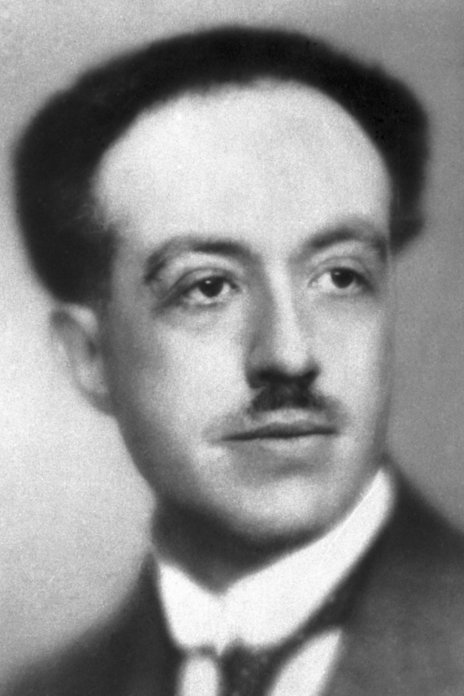
\includegraphics[height=7cm]{pic/de_Broglie.jpg}\\
\caption{\deB }
\end{figure}

\begin{figure}[!ht]
\centering
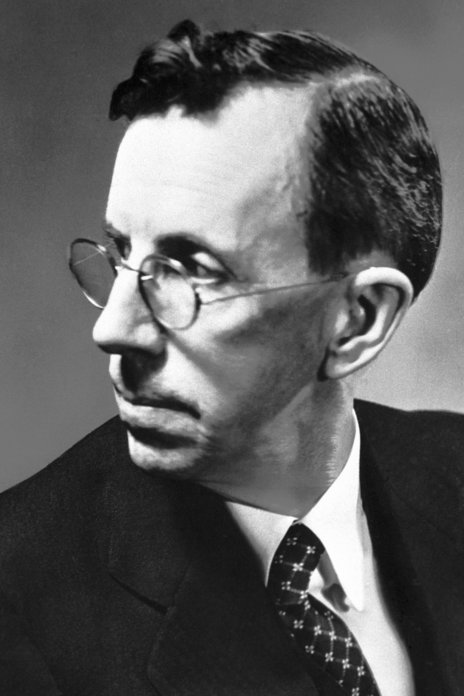
\includegraphics[height=7cm]{pic/davisson.jpg}\\
\caption{Davisson}
\end{figure}

\begin{figure}[!ht]
\centering
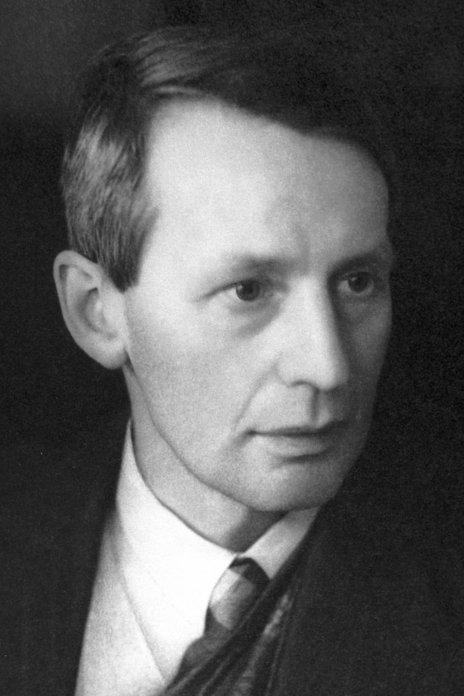
\includegraphics[height=7cm]{pic/thomson.jpg}\\
\caption{G. P. Thomson}
\end{figure}


\subsection{不确定度关系}
\begin{statT}[不确定原理]
1927年,\heisenberg 提出了微观领域的不确定原理(uncertainty principle):
有这样一些成对的可测量(例如,坐标与相应的动量分量、方位角与角动量等), 要同时测定它们的任意精确值是不可能的。其中一个量被测得越精确, 其共轭量就变得越不确定。 
\end{statT}

\begin{figure}[!ht]
\centering
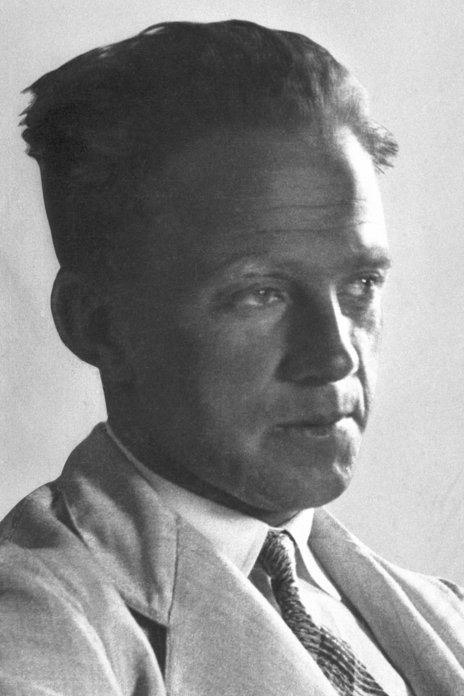
\includegraphics[height=7cm]{pic/heisenberg.jpg}\\
\caption{\heisenberg,1932年诺贝尔物理奖}
\end{figure}

\begin{figure}[!ht]
\centering
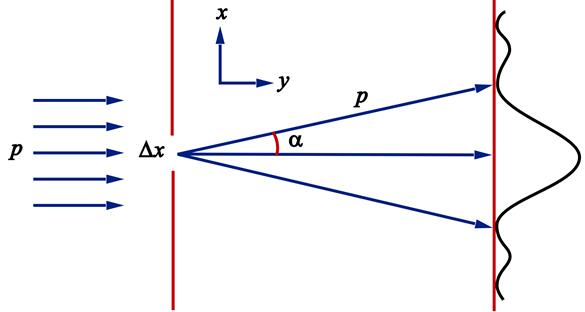
\includegraphics[height=5cm]{pic/diffraction.jpg}
\end{figure}

不确定原理可以用不同的方式来阐述, 最容易理解也最常用的是电子的单缝衍射实验:
\begin{itemize}
\item 电子通过狭缝前,动量的$x$分量$p_x$完全确定,坐标x完全不确定。
\item 电子通过狭缝后,坐标$x$的不确定度为$\delta x$,动量$p_x$的不确定度为$\delta p_x$。
\item $x$和$p_x$不可能同时精确测定,$\delta x$与$\delta p_x$之积大于或等于某个阈值。考察第一极小就能估计该阈值的大小。
\end{itemize}

\begin{figure}[!ht]
\centering
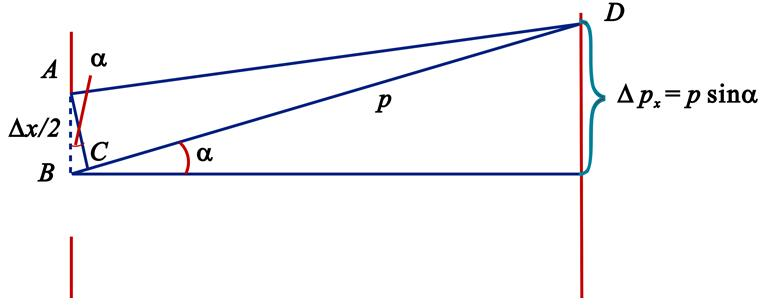
\includegraphics[height=5cm]{pic/uncertianty.jpg}
\end{figure}

点D为第一极小,
\begin{equation*}
\left.
\begin{array}{r}
\frac{\lambda}{2} = \overline{BD} - \overline{AD} \equiv \overline{BC} \approx \frac{\delta x}{2} \sin \alpha \\
\delta p_x / p = \sin \alpha
\end{array}
\right\} \implies \delta x \cdot \delta p_x = p\lambda = p(h/p) = h
\end{equation*}





\section{量子力学基本假设}

\subsection{波函数和微观粒子的状态}

\begin{exT}
某电子的波函数为:
\begin{equation*}
\phi(x) = \left\{
\begin{aligned}
ax^2+bx+c; & \text{ if } 0\le x \le 1\\
0; & \text{ otherwise}\\
\end{aligned}
\right.
\end{equation*}
请确定$a,b,c$的值:\\

\end{exT}
\begin{soluT}
根据波函数在$x=0,1$的连续性条件及波函数的归一化条件,得:
$$a=-6, b=6, c=0$$
\end{soluT}


\subsection{物理量和算符}



\subsection{本征态、本征值和}



\subsection{态叠加原理}
\begin{exT}
设$0\le x \le 1$。根据态叠加原理,波函数$\phi(x) = -6x(x-1)$可以用一组波函数$\sqrt{2}\sin n\pi x$展开成
$$\phi(x) = \sum_{n=1}^{\infty} a_n \sqrt{2}\sin n\pi x$$
的形式。试推导出$a_n$的通式。\\
提示:先证明公式$\int_{0}^{1} \left( \sqrt{2}\sin m\pi x \right) \left( \sqrt{2}\sin n\pi x \right) \D x = \delta_{mn}$ 
\end{exT}

\begin{soluT}
\begin{equation*}
\begin{array}{rl}
  & \int_{0}^{1} \left( \sqrt{2}\sin m\pi x \right) \left( \sqrt{2}\sin n\pi x \right) \D x \\
= & 2 \int_{0}^{1}\sin m\pi x \sin n\pi x \D x \\
= & 2 \int_{0}^{1} -\frac{1}{2}[cos(m+n)\pi x - cos(m-n)\pi x] \D x \\
= & \int_{0}^{1} cos(m-n)\pi x \D x \\
= & \left\lbrace 
\begin{array}{rl}
0,& \text{if  } m \ne n\\
1,& \text{if  } m = n
\end{array} \right.
\end{array}
\end{equation*}
然后来求$a_m$的通式,一方面
\begin{equation*}
\begin{array}{rl}
  & \int_{0}^{1} \left( \sqrt{2}\sin m\pi x \right) \phi(x) \D x \\
= & -6 \sqrt{2} \int_{0}^{1} \left( \sin m\pi x \right) x(x-1) \D x \\
= & -6\sqrt{2} \int_{0}^{1} x^2 \sin m\pi x \D x + 6\sqrt{2} \int_{0}^{1} x \sin m\pi x \D x \\
= & \cdots (\text{分步积分})

\end{array}
\end{equation*}
另一方面,
\begin{equation*}
\begin{array}{rl}
  & \int_{0}^{1} \left( \sqrt{2}\sin m\pi x \right) \phi(x) \D x \\
  & \int_{0}^{1} \left( \sqrt{2}\sin m\pi x \right) \left( \sum_{n=1}^{\infty} a_n \sqrt{2}\sin n\pi x \right) \D x \\
= & \sum_{n=1}^{\infty} a_n \int_{0}^{1} \left( \sqrt{2}\sin m\pi x \right) \left( \sqrt{2}\sin n\pi x \right) \D x \\
= & \sum_{n=1}^{\infty} a_n \delta_{mn} \\
= & a_m
\end{array}
\end{equation*}
\end{soluT}

\subsection{\pauli 原理}

\subsection{关于含时\schr 方程的讨论}
\begin{notationT}
为书写方便,引入符号$\hbar := \frac{h}{2\pi}$
\end{notationT}

\begin{assumpT}
波函数随时间的演化遵循含时\schr 方程:$$\I \hbar \frac{\partial}{\partial t}\Psi(x,y,z,t)=\hat{H}\Psi(x,y,z,t)$$
\end{assumpT}

\begin{corT}
考虑一种特殊形式的$\Psi(x,y,z,t)=\psi(x,y,z)f(t)$,带入含时\schr 方程,得:
$$ \hat{H}\psi(x,y,z) = E\psi(x,y,z)$$
且
$$f(t) = \exp \left(-\frac{iEt}{\hbar}\right)$$
\end{corT}

\begin{remarkT}
这一推论说明这种特殊形式的解实际上是一种驻波,即各处以固定的(不随时间变化的)振幅做振动。而定态的\schr 方程实际描述的是这种驻波的振幅$\psi(x,y,z)$。
\end{remarkT}

\begin{proof}
将$\Psi(x,y,z,t)=\psi(x,y,z)f(t)$,带入含时\schr 方程,得:
\begin{equation*}
\begin{aligned}
\I \hbar \frac{\partial}{\partial t}\left( \psi(x,y,z)f(t)\right) & = \hat{H}\psi(x,y,z)f(t) \\
\I \hbar \frac{1}{f(t)} \frac{\D f(t)}{\D t}  & = \frac{\hat{H}\psi(x,y,z)}{\psi(x,y,z)}
\end{aligned}
\end{equation*}
注意到左边只与时间变量$t$有关,而右边只与空间坐标$x,y,z$有关,唯一的可能性两者左右两边都等于一个常数$E$。于是右边给出
$$ \hat{H}\psi(x,y,z) = E\psi(x,y,z)$$
正是定态的\schr 方程,而左边给出
$$ \I \hbar \frac{\D f(t)}{\D t} = E f(t) $$
其解为:
$$f(t) = \exp \left(-\frac{iEt}{\hbar}\right)$$










\end{proof}





\section{箱中粒子的\schr 方程及其解}

\subsection{箱中粒子}



\subsection{应用}


